\section{Fake-$\thad$ scale factor calibration in the CRtt}
\label{sec:tauFF_appendix}

Figure~\ref{fig:ttCR_mtt} presents the post-fit distributions of the leading $\thad$ $\pt$ in the CRtt. These show good agreement between the data and the fitted background model.
Tables~\ref{tab:ff1_summary} and~\ref{tab:ff2_summary} summarise the scale factors for 1-prong and 3-prong fake $\tau$ decays
derived from the CRtt including both the statistical and systematic uncertainties. However, the interpretation of these scale factors is difficult due to their large correlations. 

\begin{figure}[H]
\centering
\begin{tabular}{@{}ccc@{}}
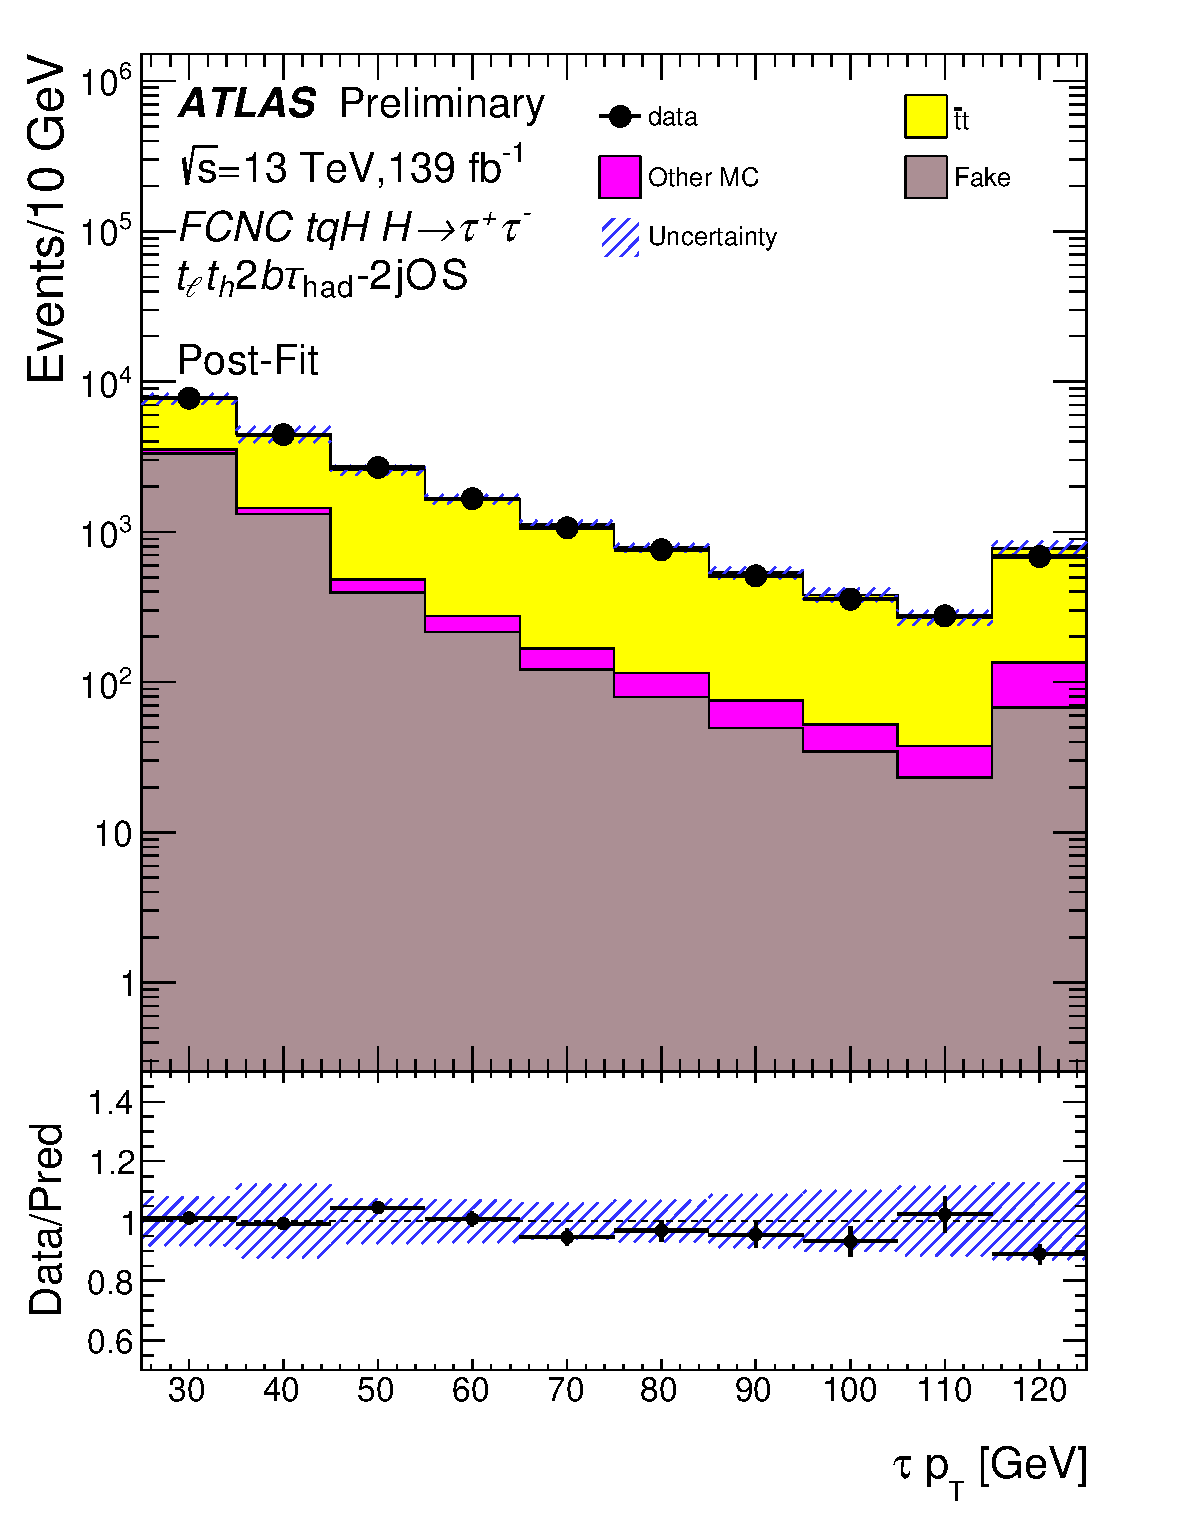
\includegraphics[page=1,width=0.29\textwidth]{figures/ttCR/tuH_reg1l1tau2b2j_os_log_ttCR.pdf} &
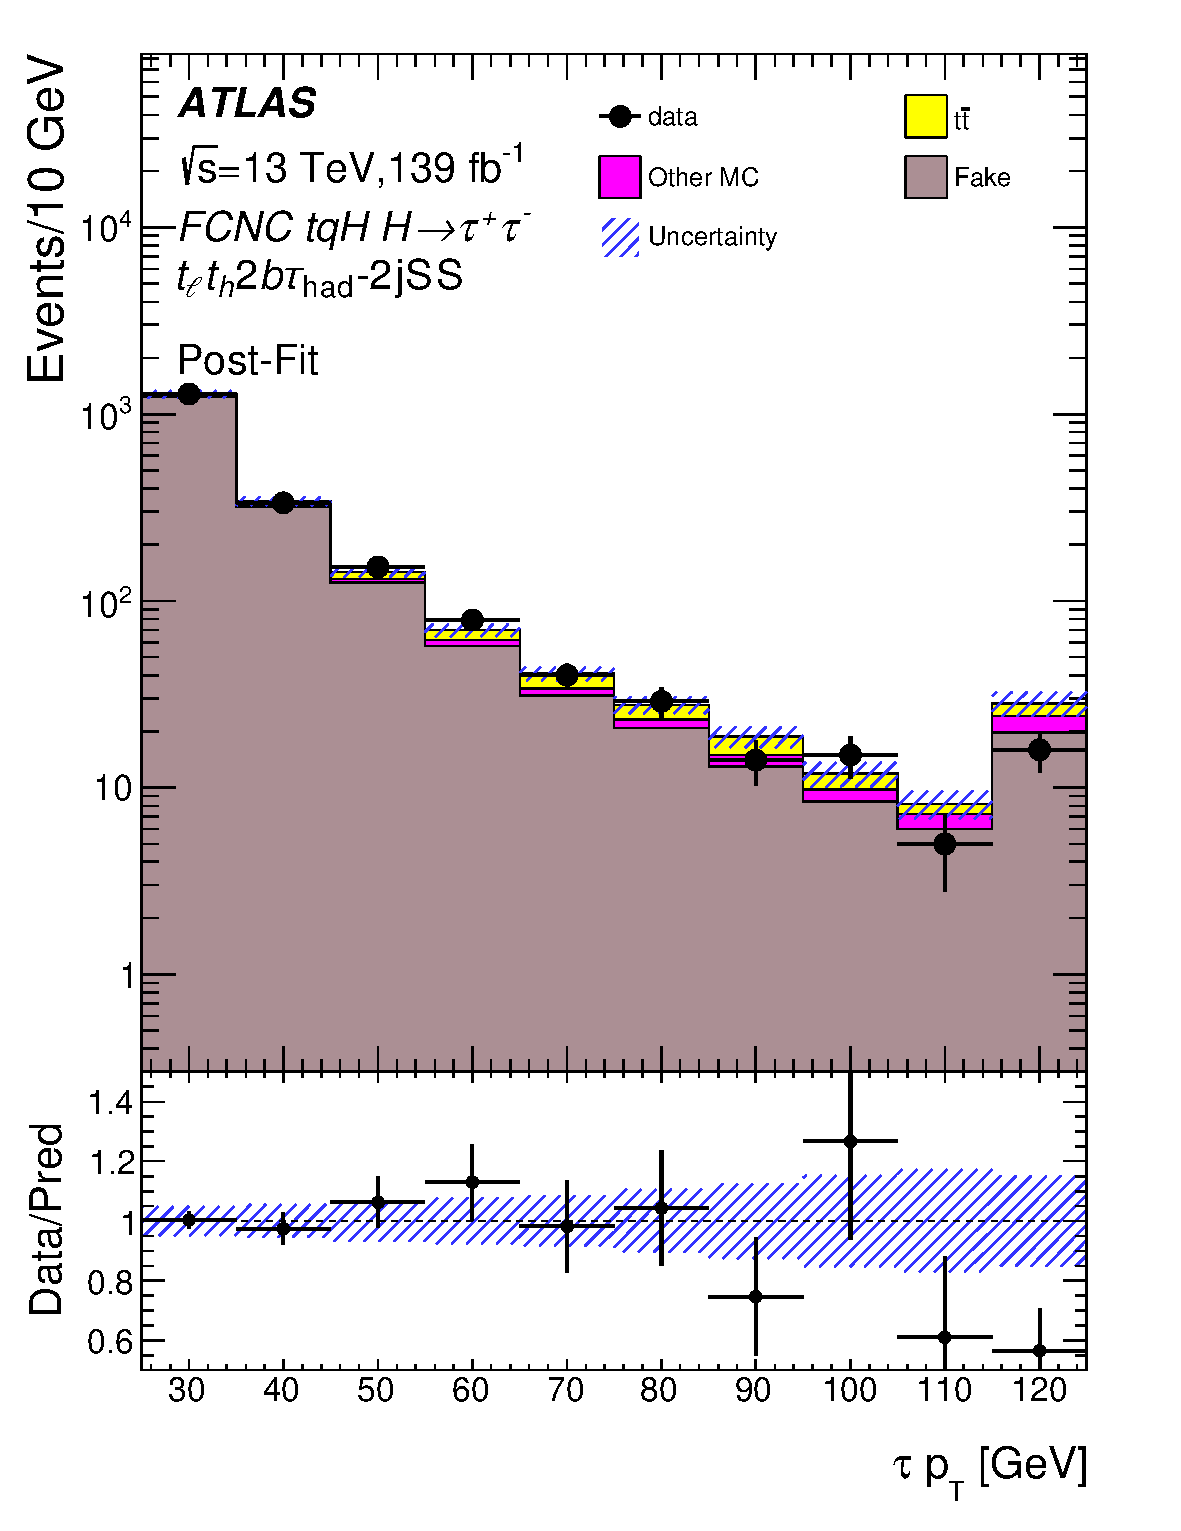
\includegraphics[page=1,width=0.29\textwidth]{figures/ttCR/tuH_reg1l1tau2b2j_ss_log_ttCR.pdf}&
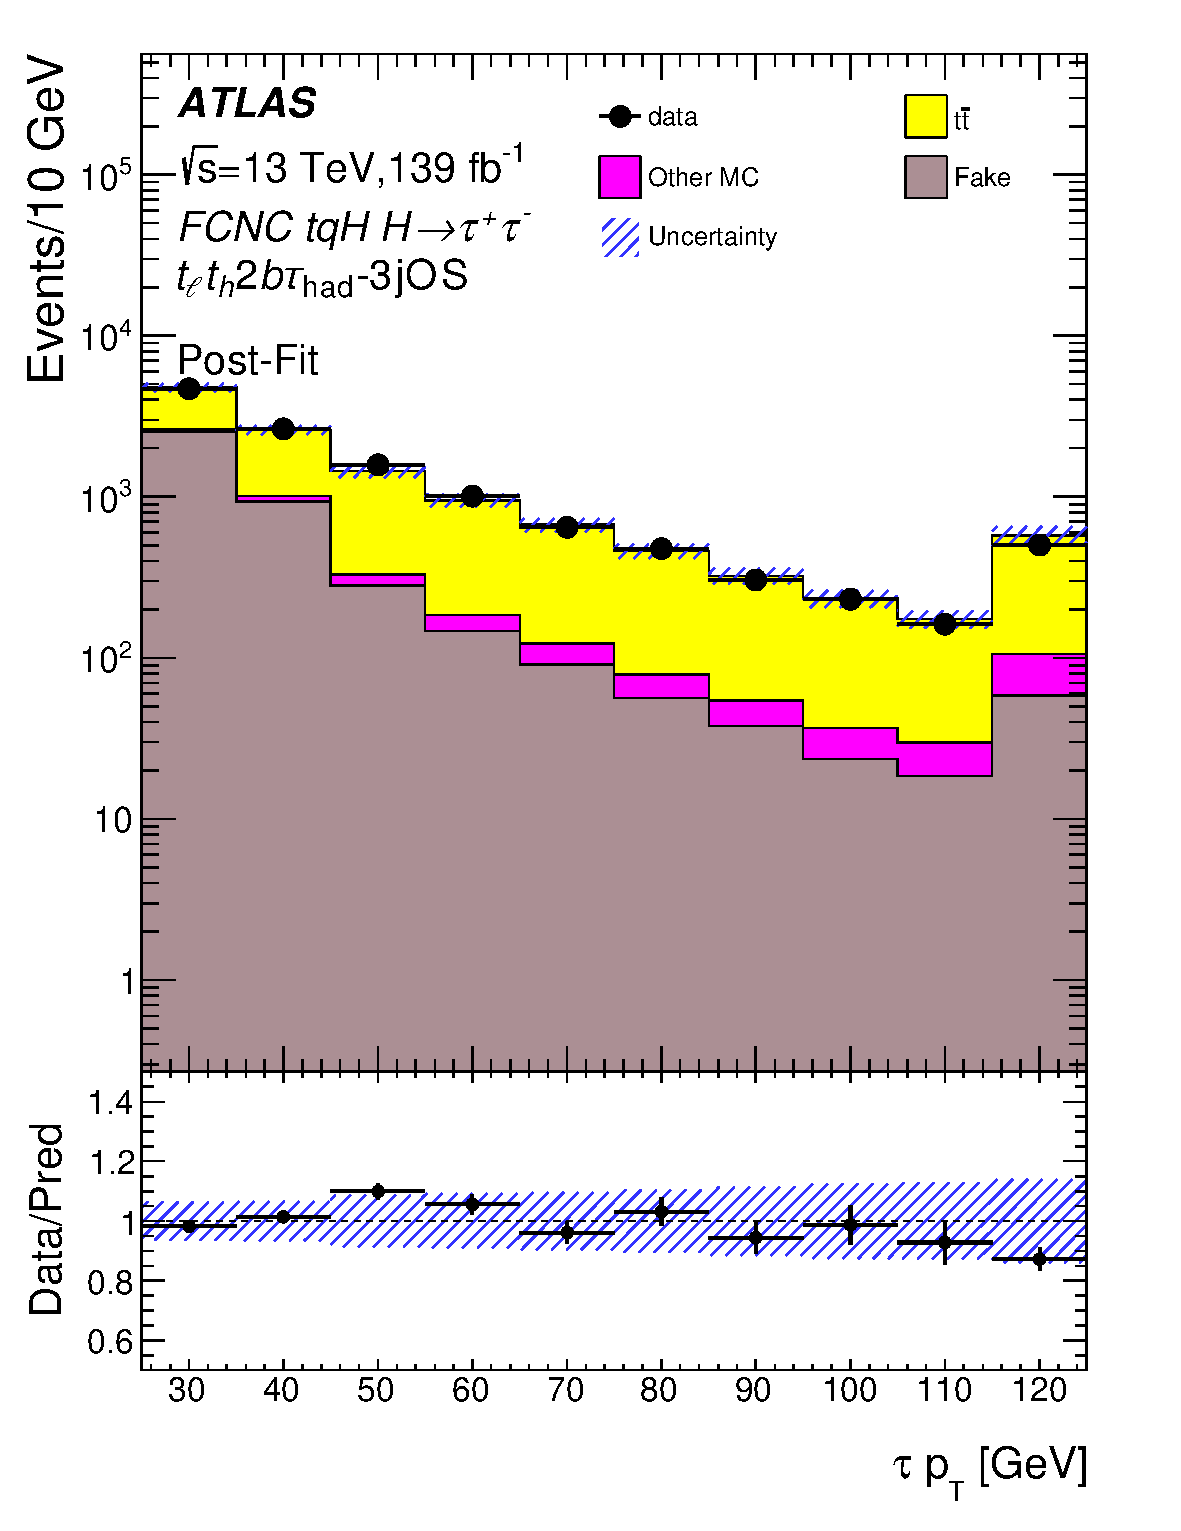
\includegraphics[page=1,width=0.29\textwidth]{figures/ttCR/tuH_reg1l1tau2b3j_os_log_ttCR.pdf}\\
(a) & (b) & (c) \\
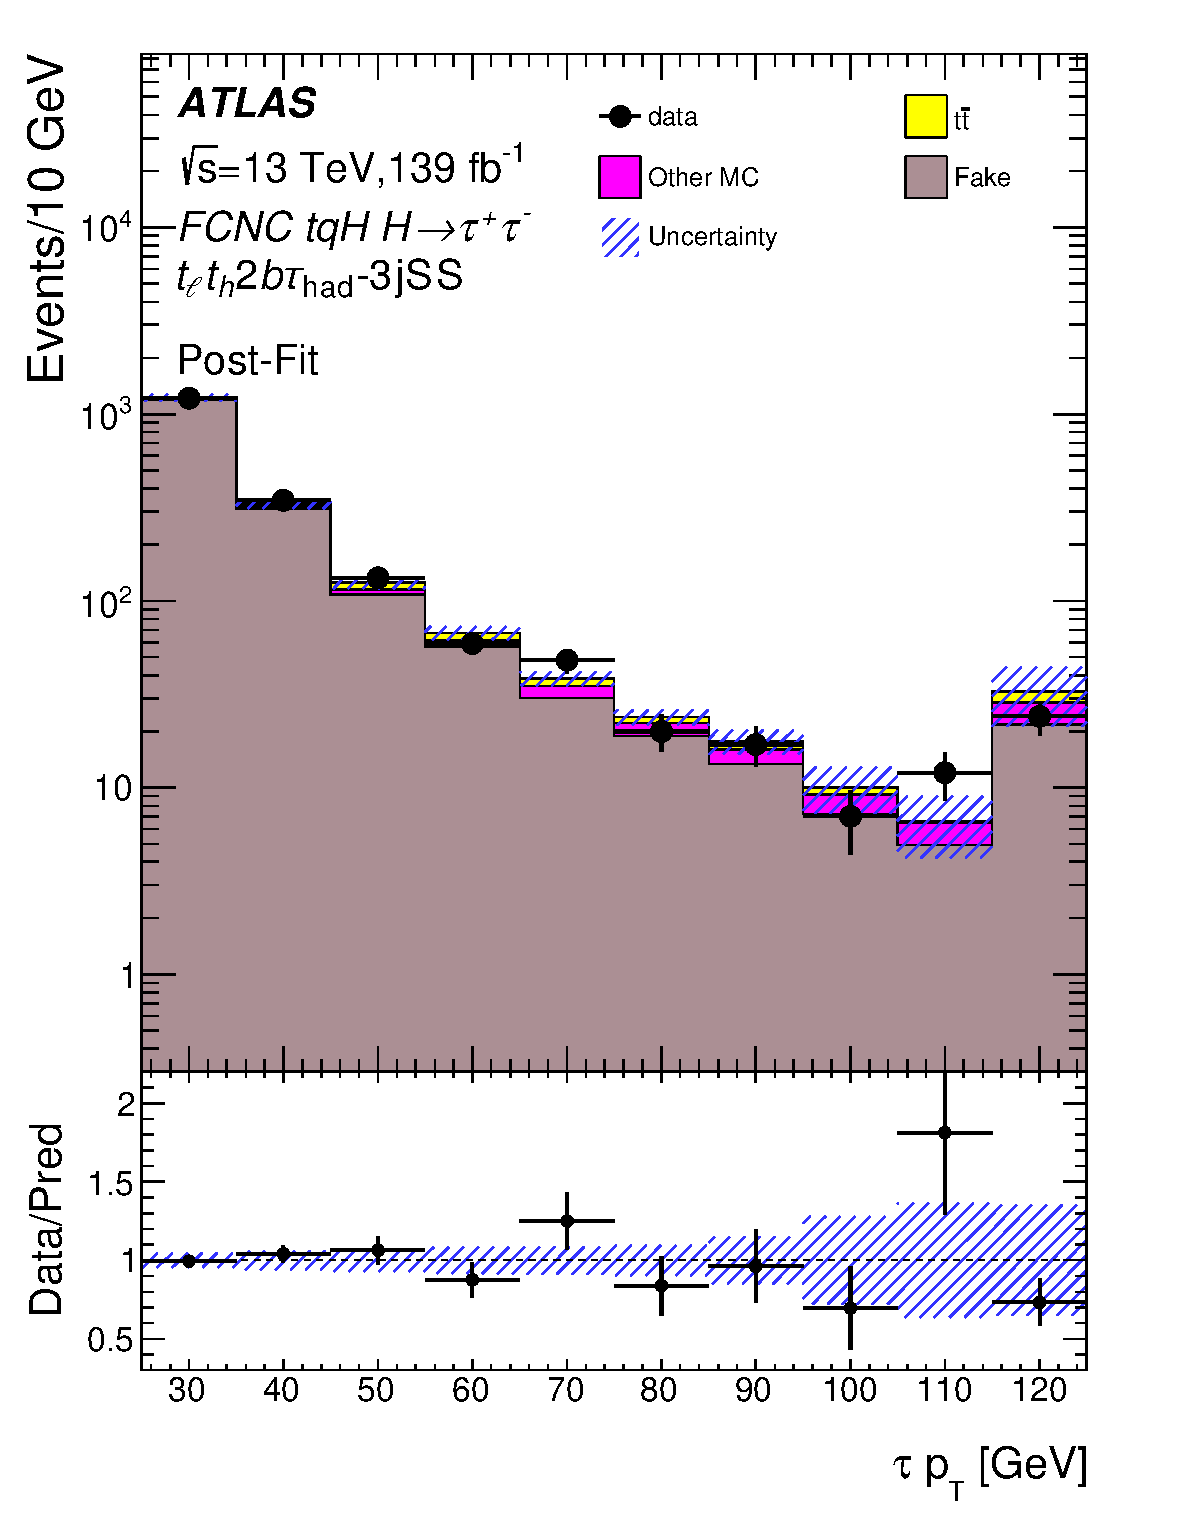
\includegraphics[page=1,width=0.29\textwidth]{figures/ttCR/tuH_reg1l1tau2b3j_ss_log_ttCR.pdf}&
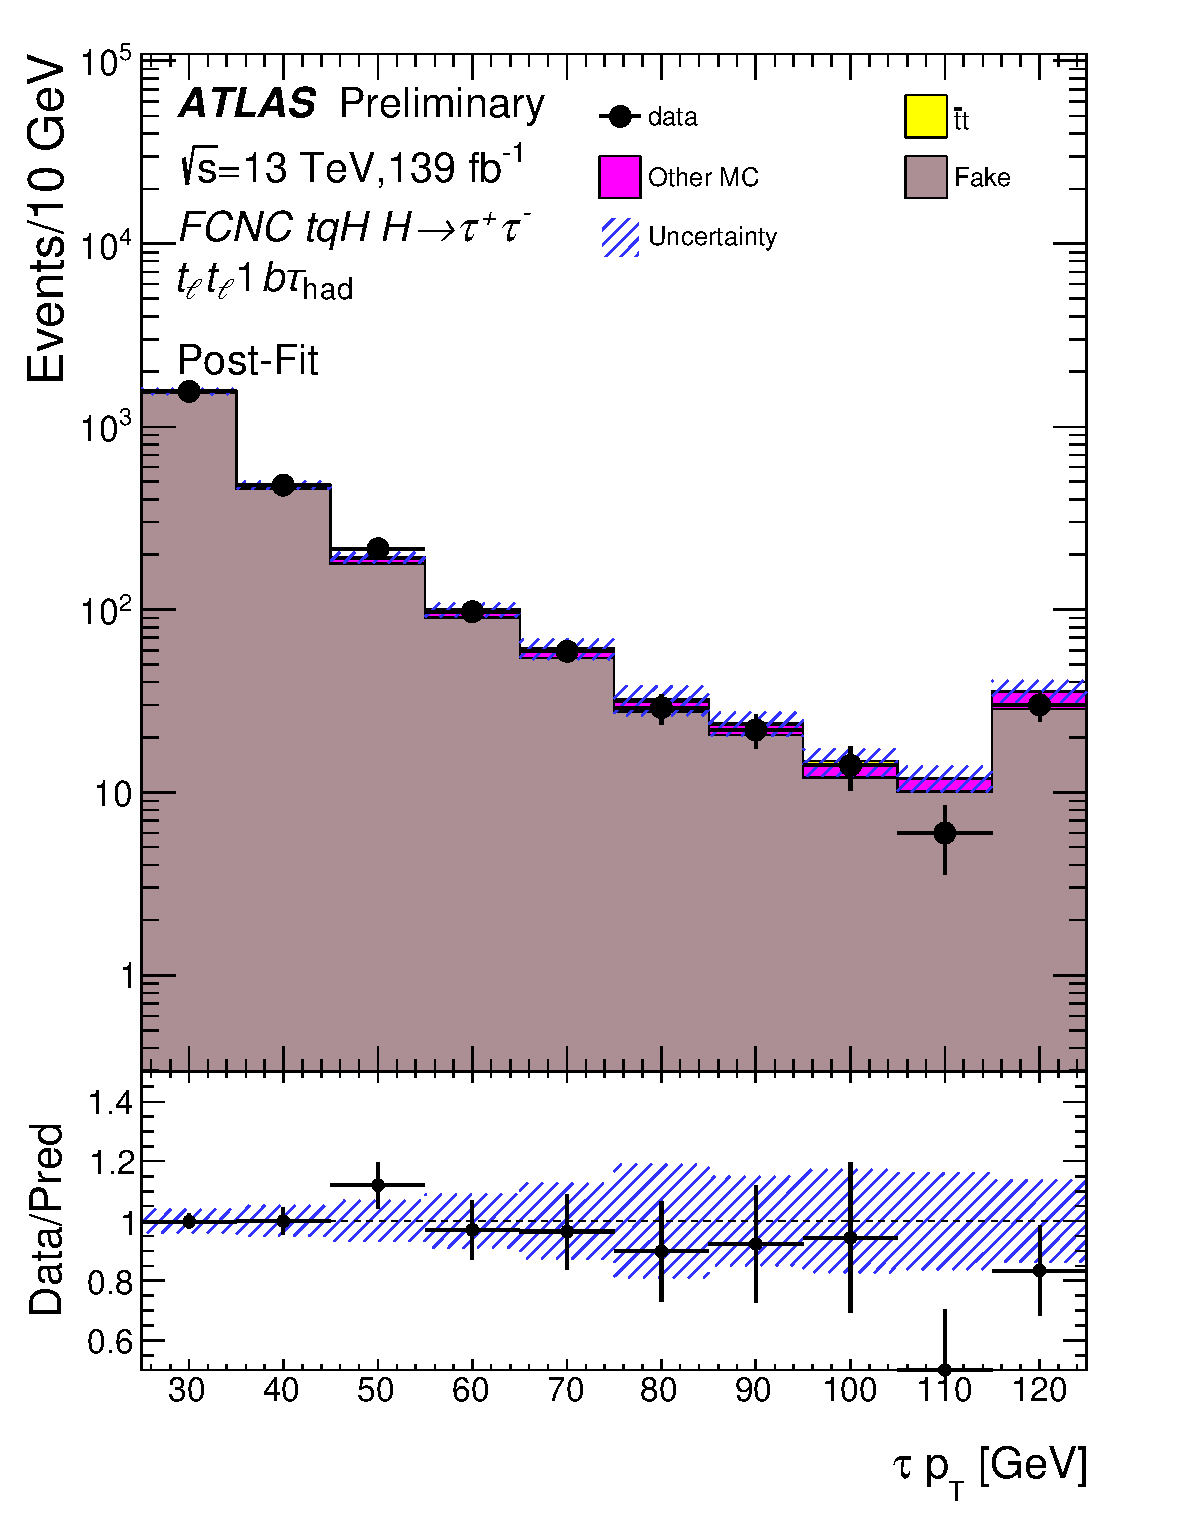
\includegraphics[page=1,width=0.29\textwidth]{figures/ttCR/tuH_reg2l1tau1bnj_log_ttCR.pdf}&
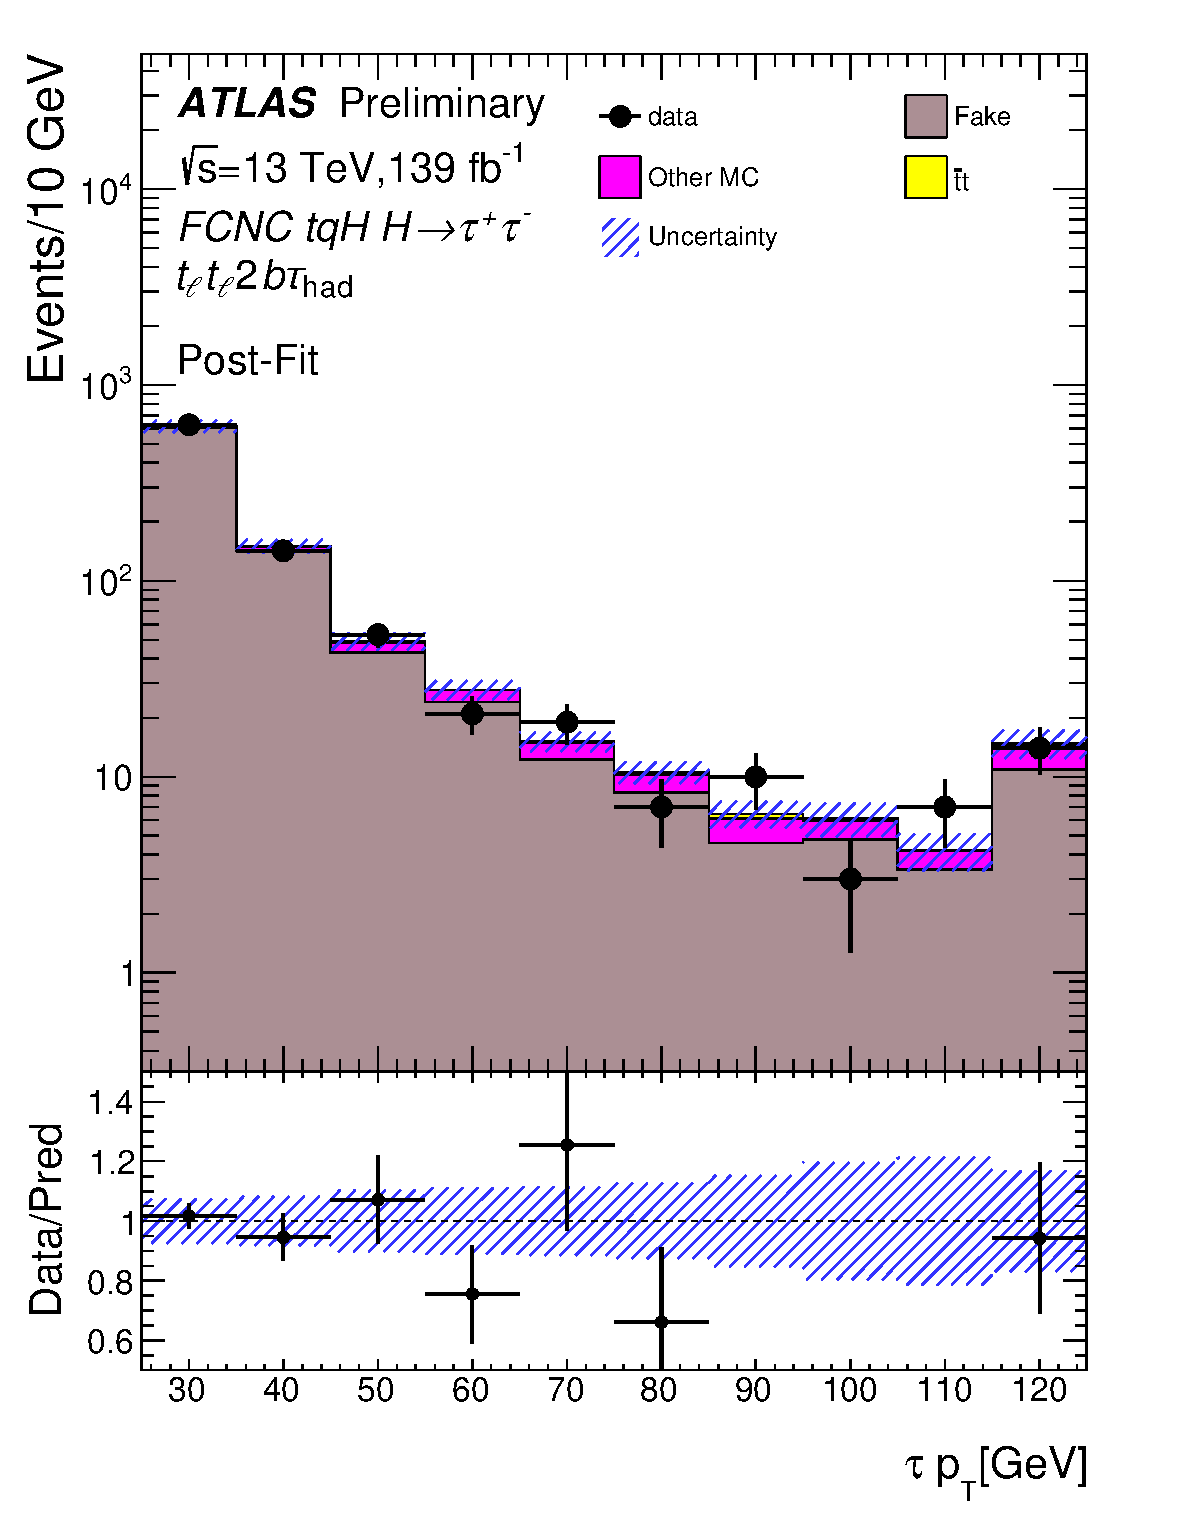
\includegraphics[page=1,width=0.29\textwidth]{figures/ttCR/tuH_reg2l1tau2bnj_log_ttCR.pdf}\\
(d) & (e) & (f)\\
\end{tabular}
\caption{Leading $\thad$ $\pt$  distributions obtained after the fit to data (`Post-Fit') for the fake-$\thad$ scale factors in the following CRtt:
  (a) $t_{\ell}t_{h}$2b$\thad$-2j OS, (b) $t_{\ell}t_{h}$2b$\thad$-2j SS, (c) $t_{\ell}t_{h}$2b$\thad$-3j OS, (d) $t_{\ell}t_{h}$2b$\thad$-3j SS,
  (e) $t_{\ell}t_{\ell}$1b$\thad$-nj and (f) $t_{\ell}t_{\ell}$2b$\thad$-nj.
  The total statistical and systematic uncertainty of the background prediction is indicated by the hatched band.
  Overflow events are included in the last bin. The lower panels show the ratio of data to prediction.}
\label{fig:ttCR_mtt}
\end{figure}

\begin{table}
\caption{ Summary of fake-$\tau$ (1-prong) scale factors derived in the CRtt. The numbers are shown as central values, statistical uncertainties, and systematics uncertainties. }
\begin{center}
\begin{tabular}{lcccccc}
\toprule\toprule

Fake-$\tau$ types & \multicolumn{3}{c}{1-prong $\tau$ decay}  \\ \midrule
$\thad$ $\pt$                                   &  25--35~\GeV  & 35--45~\GeV  &  $>45$~\GeV            \\
\midrule
Type-1                          &$0.71 \pm 0.01 \pm 0.03 $ &$0.61 \pm 0.02 \pm 0.04 $ &$0.38 \pm 0.02 \pm 0.05 $  \\
% W fake OS
Type-2                          &$0.76 \pm 0.06 \pm 0.04 $ & $0.37 \pm 0.08 \pm 0.02$ & $0.74 \pm 0.08 \pm 0.02 $ \\
% W fake SS
Type-3                          &$0.62 \pm 0.10 \pm 0.03 $ &$0.83 \pm 0.09 \pm 0.03 $ &$0.94 \pm 0.07 \pm 0.02 $  \\
%  b fake
Type-4                          &$1.20 \pm 0.02 \pm 0.01 $ & $1.01 \pm 0.04 \pm 0.02 $ &$0.76 \pm 0.03 \pm 0.03 $  \\
% other fake
\bottomrule\bottomrule
\end{tabular}
\label{tab:ff1_summary}
\end{center}
\end{table}


\begin{table}
\caption{ Summary of fake-$\tau$ (3-prong) scale factors derived in the CRtt. The numbers are shown as central values, statistical uncertainties, and systematics uncertainties. }
\begin{center}
\begin{tabular}{lcccccc}
\toprule\toprule

Fake-$\tau$ types        & \multicolumn{3}{c}{3-prong $\tau$ decays}  \\ \midrule
$\thad$ $\pt$                             &  25--35~\GeV  & 35--45~\GeV       &  $>45$~\GeV  \\
\midrule
Type-1                                    & $1.01 \pm 0.03 \pm 0.04 $ & $1.09 \pm 0.04 \pm 0.05 $ & $0.30 \pm 0.05 \pm 0.07 $ \\
% W fake OS
Type-2                                    & $0.93 \pm 0.10 \pm 0.04 $ & $1.05 \pm 0.09 \pm 0.03 $ & $0.79 \pm 0.09 \pm 0.04 $ \\
% W fake SS
Type-3                                    & $1.07 \pm 0.13 \pm 0.03 $ &$1.39 \pm 0.12 \pm 0.03 $ &$1.26 \pm 0.10 \pm 0.04 $  \\
%  b fake
Type-4                                    &$1.28 \pm 0.07 \pm 0.02 $ &$0.66 \pm 0.08 \pm 0.01 $ & $0.71 \pm 0.07 \pm 0.02 $ \\
% other fake
\bottomrule\bottomrule
\end{tabular}
\label{tab:ff2_summary}
\end{center}
\end{table}


